\section{Chapter 5 - Problem (11)}
	You must push a crate across a floor to a docking bay. The crates weighs $180 \ lb$. The coefficient of static friction between crate and floor is $0.57$, and the coefficient of kinetic friction is $0.35$. Your force on the crate is directed horizontally.

	\subsection{Question (a)}
		What magnitude of your push puts the crate on the verge of sliding?

		\textbf{R:} \newline

		\begin{figure}[H]
			\begin{center}
				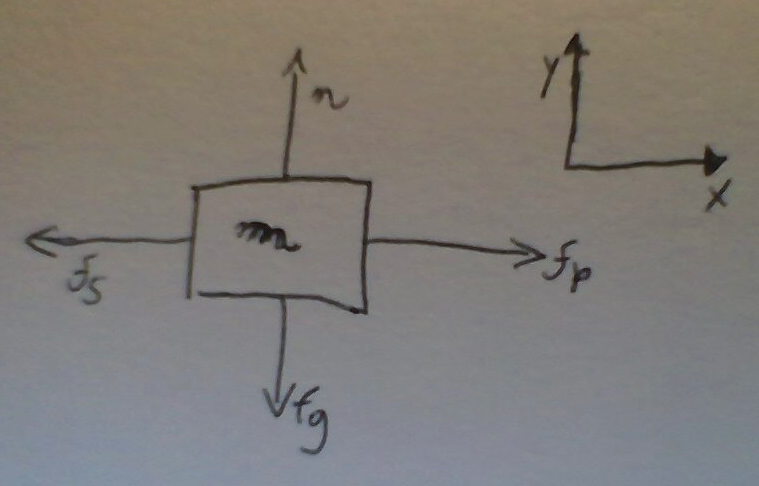
\includegraphics[scale=0.3]{hw6_problemb_a_fbd}
				\caption{Free-Body Diagram (Problem 11 (a))}
				\label{fig:hw6_problemb_a_fbd}
			\end{center}
		\end{figure}

		\begin{align}
			f_{s} = \ &f_{s_{max}} = \mu_{s}n& \notag
		\end{align}

		Newton's $2^{nd}$ Law to discover $n$:

		\begin{align}
			\sum F_{y} = \ &ma_{y}& \notag \\
			n - f_{g} = \ &m(0)& \notag \\
			n = &f_{g}& \notag
		\end{align}

		\begin{align}
			f_{s} = \ &(0.57)(180 \ lb)& \notag \\
			= \ &102.6 \ lb&
		\end{align}

		The push needs to be greater than $102.6 \ lb$ in order to slide the crate.

	\subsection{Question (b)}
		With what magnitude must you then push to keep the crate moving at a constant velocity?

		\textbf{R:} \newline

		\begin{figure}[H]
			\begin{center}
				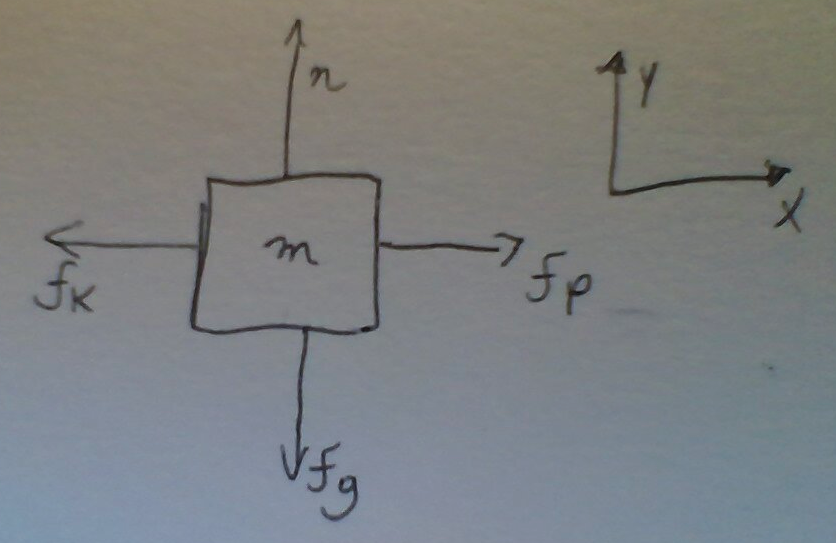
\includegraphics[scale=0.3]{hw6_problemb_b_fbd}
				\caption{Free-Body Diagram (Problem 11 (b))}
				\label{fig:hw6_problemb_b_fbd}
			\end{center}
		\end{figure}

		\begin{align}
			f_{k} = \ &\mu_{k}n& \notag \\
			= \ &(0.35)(180 \ lb)& \notag \\
			= \ &63 \ lb&
		\end{align}

		The push needs to be exactly $63 \ lb$ in order to keep the crate moving at a constant velocity.

	\subsection{Question (c)}
		If, instead, you then push with the same magnitude as the answer to \emph{(a)}, what is the magnitude of the crate's acceleration?

		\textbf{R:} \newline

		Newton's $2^{nd}$ Law:
		\begin{align}
			\sum F_{x} = \ &ma_{x}& \notag \\
			f_{p}-f_{k} = \ &ma& \notag \\
			m = \ &\frac{f_{g}}{g}& \notag \\
			= \ &\frac{180 \ lb}{32.2 \ ft/s^{2}} = 5.59 \ sl& \notag \\
			a = \ &\frac{f_{p}-f_{k}}{m}& \notag \\
			= \ &\frac{(102.6 \ lb)-(63 \ lb)}{5.59 \ sl}& \notag \\
			= \ &7.084 ft/s^{2}&
		\end{align}
